\documentclass[aps,pre,twocolumn,letterpaper,floatfix,nofootinbib]{revtex4}
	% for \code color
\usepackage[dvipsnames]{xcolor}
\usepackage{graphicx}
\usepackage{amsmath,amssymb,amsfonts}
\usepackage{mathtools}
\usepackage{pdfpages}
\usepackage{afterpage}
\usepackage[hidelinks]{hyperref}
\usepackage{epstopdf}
\usepackage{todonotes}
\usepackage{menukeys}
\usepackage{siunitx}
\usepackage{listings}
% Pretty formating of c++ (see \cpp command)
\usepackage{xspace}
\newcommand*{\cpp}{C\ensuremath{++}\xspace}

\lstdefinelanguage{LAMMPS}{
    morekeywords={units,atom_style,lattice,region,create_box,create_atoms,pair_style,pair_coeff,neigh_modify,mass,velocity,fix,run, group every, equal, count, porosity, EDGE},
    sensitive=false, % keywords are not case-sensitive
    morecomment=[l]{//}, % l is for line comment
    morecomment=[s]{/*}{*/}, % s is for start and end delimiter
    morestring=[b]" % defines that strings are enclosed in double quotes
}

\lstset{
numbers=left,
numberstyle=\small,
numbersep=8pt,
frame = single,
language=LAMMPS,
framexleftmargin=15pt,
xleftmargin=0.65cm,
xrightmargin=0.1cm}

% Highlighte inline code
\definecolor{light-gray}{gray}{0.95}
\definecolor{atomify-red}{rgb}{0.90196078 , 0.09803922, 0.29411765}
\definecolor{atomify-green}{rgb}{0.23529412 , 0.70588235, 0.29411765}
\definecolor{atomify-yellow}{rgb}{0.8,  0.70588235,  0.07843138}
\definecolor{atomify-blue}{rgb}{0.00000000 , 0.50980392, 0.78431373}
%\newcommand{\code}[1]{\mbox {\texttt{#1}}}
\newcommand{\code}[1]{\colorbox{light-gray}{\color{RawSienna}\texttt{#1}}}

\begin{document}

\title{Increased productivity using Atomify - a real-time LAMMPS visualizer}
\author{Anders Hafreager$^1$}
\author{Svenn-Arne Dragly$^{1}$}
%\author{Anders Malthe-S\o renssen$^1$}
\affiliation{$^1$Department of Physics - University of Oslo\\Sem S{\ae}lands vei 24, NO-0316, Oslo, Norway }
\date{\today}

%%%%%%%%%%%%%%%%%%%%%%%%%%%%%%%%%%%%%%%%%%%%%%%%%%%%%%%%%%%%%
%%%%%%%%%%%%%%%%%%%%%%%%%%%%%%%%%%%%%%%%%%%%%%%%%%%%%%%%%%%%%

\begin{abstract}
%
The typical workflow when running atomistic simulations includes working with several programs.
A text editor is needed to create and modify the scripts, the terminal to run the simulation, and programs like VMD or Ovito to visualize the system over time.
If physical quantities are computed, the data is often plotted using programming languages like MATLAB or Python,
where additional scripts must be used.
This is a tedious process, especially for teaching purposes and for people who are new in the field.
We here introduce Atomify; a high performance real-time visualizer for atomistic simulations that can simulate and render more than one million atoms with excellent frame rate on modern hardware.
Atomify supports OpenMP acceleration, GPU acceleration, real-time plotting of physical quantities, and an easy-to-use code editor in one single application.
It currently uses LAMMPS as physics engine, but it can be extended to support other codes like Gromacs, NAMD or OpenMM.
Atomify is open-source software (GPL) written in C++ using the Qt framework.
%
\end{abstract}

\maketitle

\section{Introduction}

Over the past decades, users of LAMMPS\citep{Plimpton1995Fast} and other molecular dynamics simulators such as GROMACS, NAMD and CHARMM\citep{berendsen1995gromacs, Phillips2005Scalable, brooks2009charmm} have
typically written scripts in a text editor and run the scripts by passing them to the simulator
on the command line.
The simulator in turn writes the results to disk and the user analyzes the results
by reading the files manually or passing them to other programs.
With the arrival of software like VMD,\citep{Humphrey1996Vmd}
it become easy to both visualize the trajectories and certain physical quantities.
VMD came with support both for reading the results from file or attaching to a
running process of supported simulators.
Later, modern visualization tools like Ovito\citep{Stukowski2009Visualization} has made both visualization and analysis more
accessible to new users through its powerful scriptable modifier pipeline.
In addition, the results can be loaded into common programming languages like MATLAB and Python
to produce publication-ready figures.

In combination, the text editors, the simulators, the visualization software, and the programming
languages like MATLAB and Python define the workflow of a typical researcher in computational
materials science.
While this is a powerful workflow in well-established simulations,
it is tedious for prototyping new ideas.
The workflow requires a fairly large amount of context switching,
moving from the text editor to the terminal to run the simulation,
waiting for the results, and then finally being able to study them using the analysis
and visualization tools.

Here, we present Atomify, a software that integrates script editing,
visualization and analysis into one tool.
Atomify has detailed knowledge about the inner workings of LAMMPS,
which makes it capable not only of visualizing the simulation results,
but also how the simulation is defined in terms of different groups and regions.

It is especially useful during development of new scripts, but can be used
to run full, publication-ready simulations with minimal simulation overhead.

\begin{figure*}
	\centering
	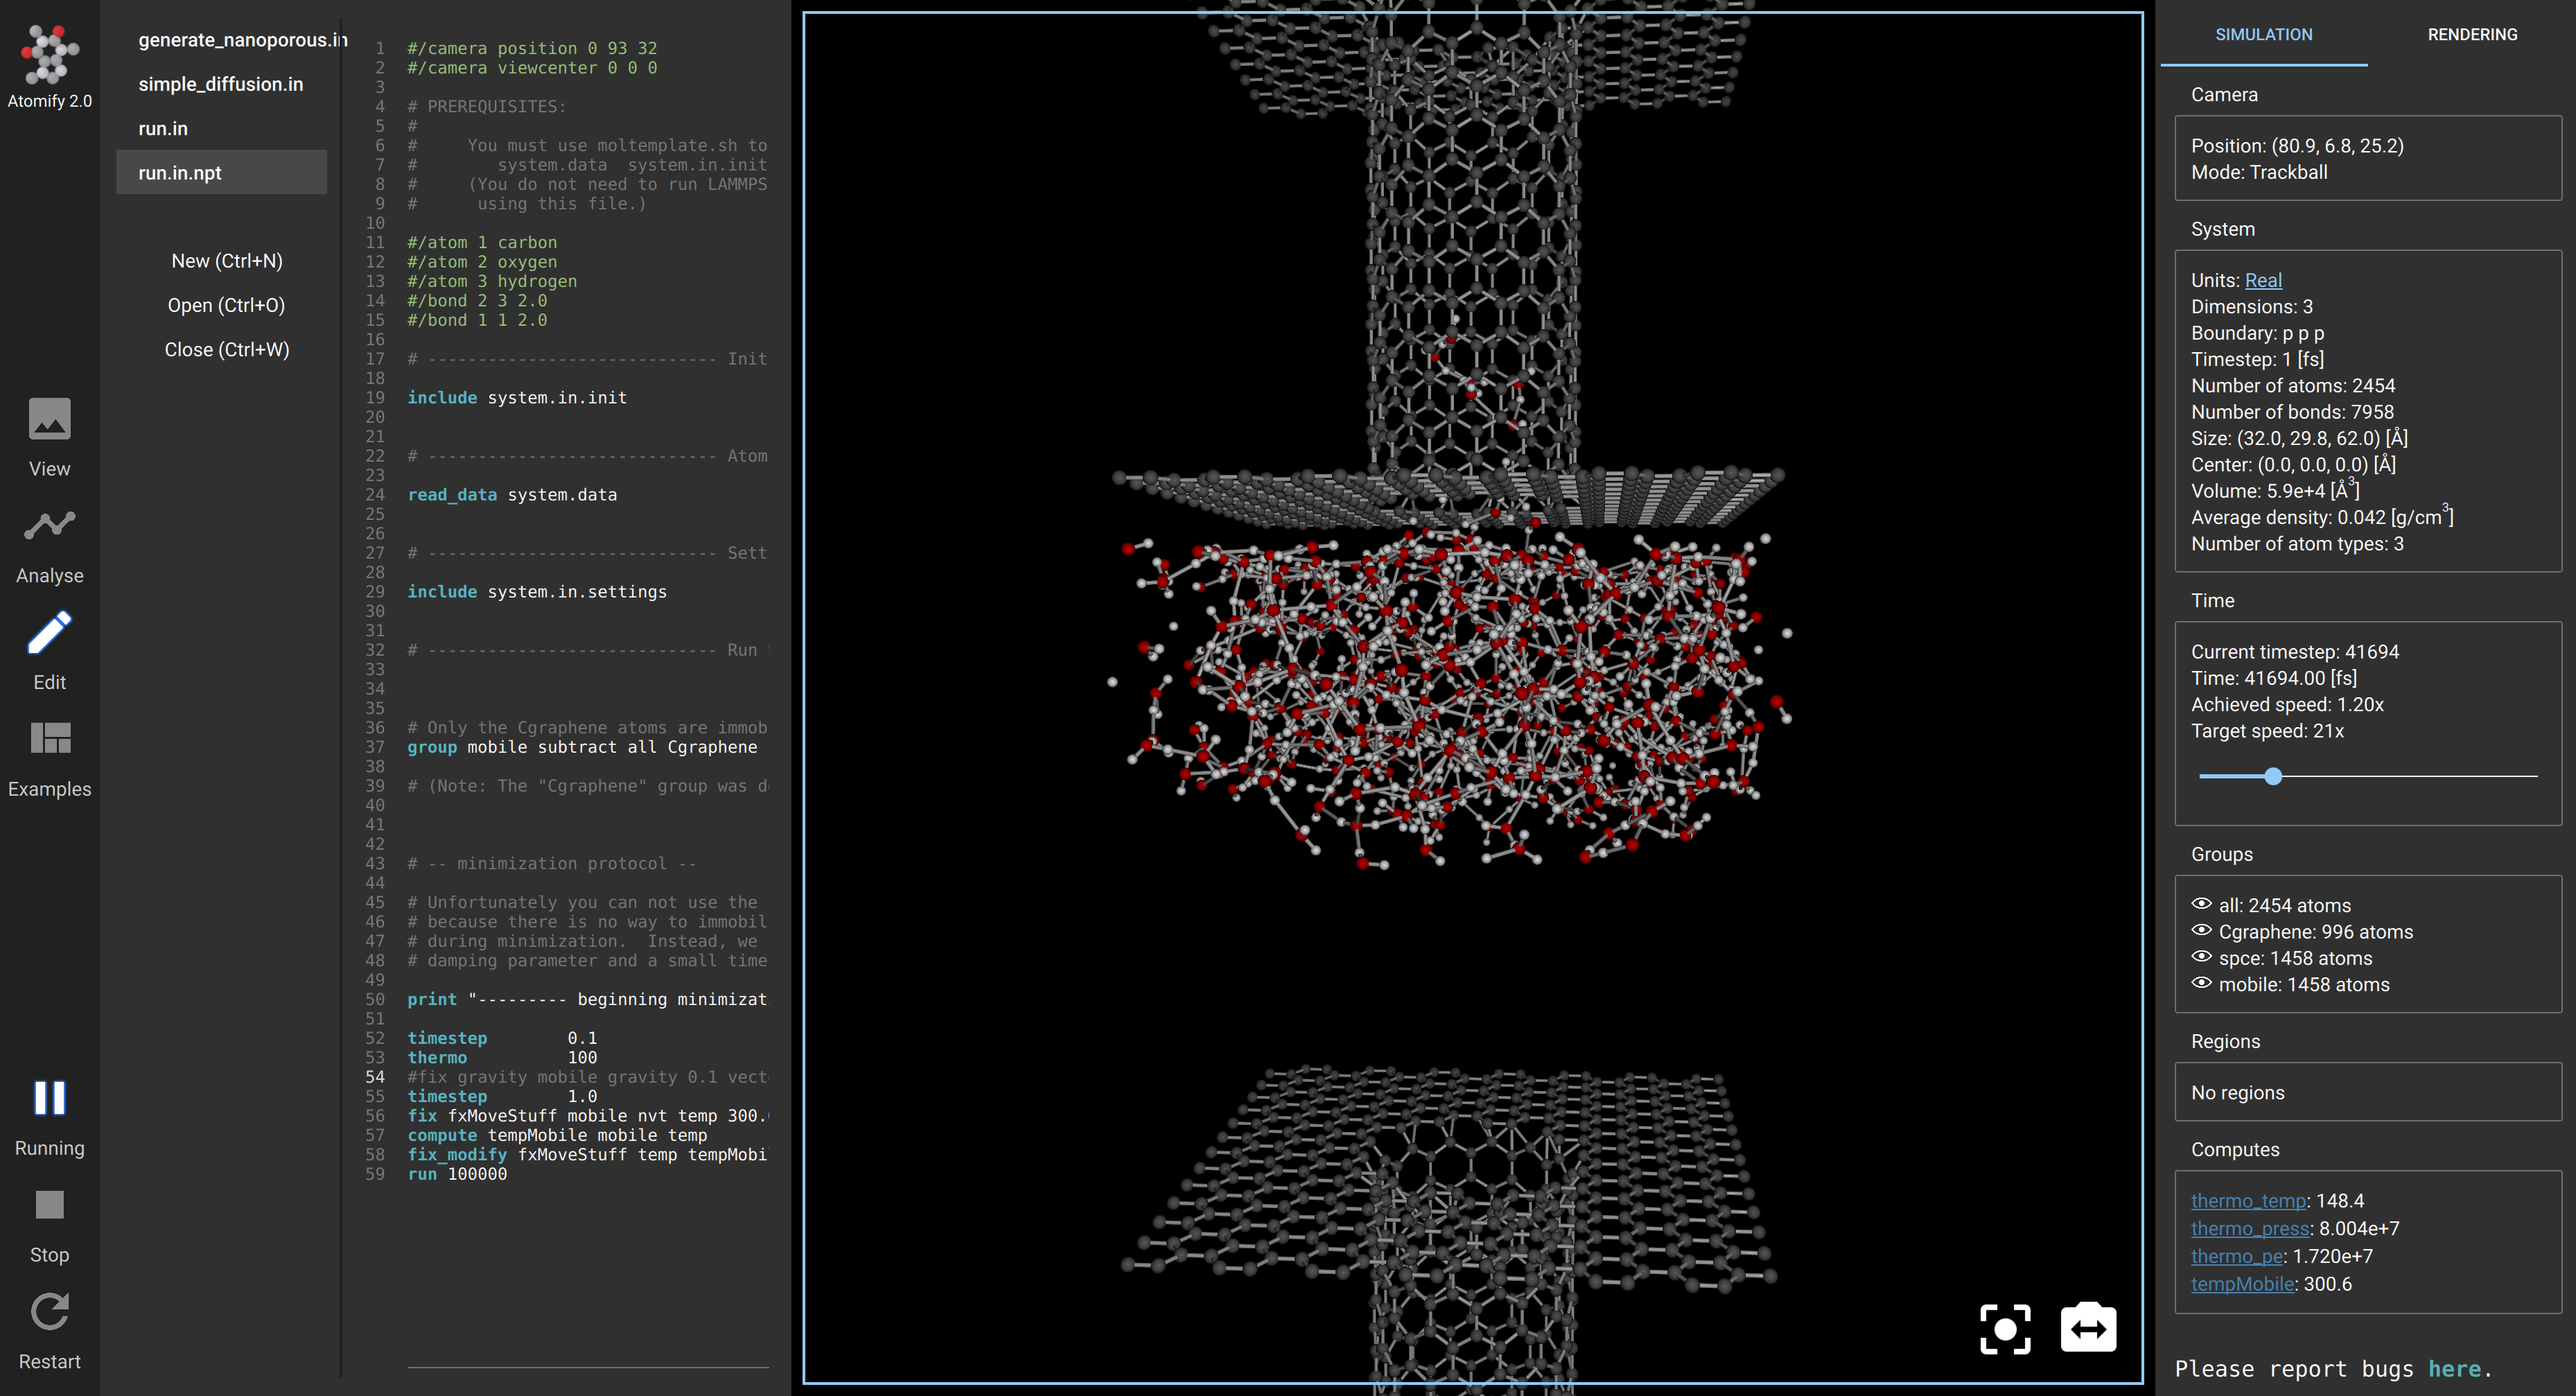
\includegraphics[width=\textwidth]{gui.png}
	\caption{%
    Overview of the Graphical User Interface (GUI) in Atomify.
    The toolbar (1) is used to change between the different modes, such as
    editing, viewing and analyzing the running simulation,
    in addition to playback controls.
    The file browser (2) contain the list of open LAMMPS scripts or data files.
    The text editor (3) provides code highlighting.
    The viewport (4) shows the current simulation.
    The simulation properties (5) shows the simulations details, gives access to
    LAMMPS objects such as groups, regions and computes, and the rendering
    properties (6) lets you change the viewport settings, such as lighting and
    draw mode.
    TODO: Add numbers to figure.
    }
	\label{fig:gui}
\end{figure*}

In this paper we will go through a case study, an example simulation, where we
use many of the useful features Atomify provides.
We start by discussing the GUI in section \ref{sec:features} where the main features are summarized.
In section \ref{sec:casestudy}, the case study is introduced where we go through a typical example
of a simulation that uses regions and groups to perform different integration on different atoms.
Common pitfalls which are easily picked up with Atomify are shown.

\section{\label{sec:features}Summary of features}
Atomify was designed to improve workflow with reduced number of
context switches and mouse clicks to obtain immediate results from a simulation.
Its main features can be summarized as script editing,
real-time visualization and plotting of physical quantities.
This turns out to improve the workflow substantially.
In addition, Atomify comes with multiple examples,
many of which have been made by members of the LAMMPS community.

\begin{figure}
	\centering
	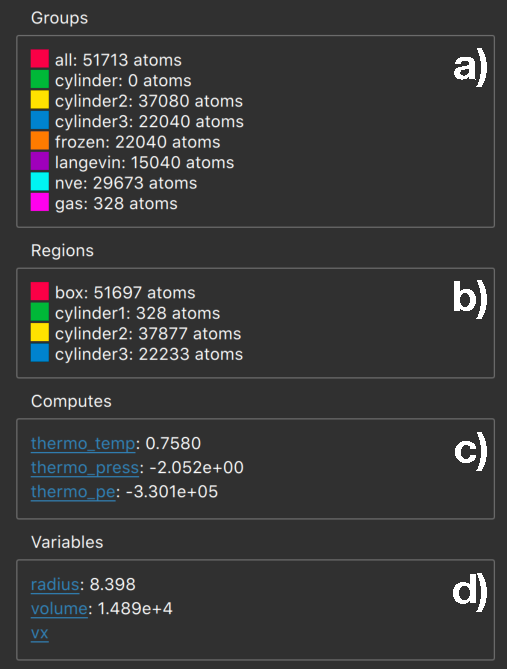
\includegraphics[width=0.5\textwidth]{figures/rightbar.pdf}
	\caption{
		The \textit{Simulation summary} is a powerful feature in Atomify where relevant
		properties from LAMMPS is presented real-time.
		In a), a list of all groups defined is shown with the current atom count.
		b) shows all defined regions. Each group and region can be hovered so that atoms
		are colored after what group / region they are in. If an atom is in multiple
		groups or regions, they will get the color of the latest one defined.
		The color boxes can be clicked which will either always highlight the atoms in a certain group or region,
		or if clicked again, hide all of them.
		In c) and d), a list of all variables and computes is shown. If a variable or compute
		produces a scalar, the current value is shown as can be seen with all the variables.
		By clicking the name, a plot will show up showing the time evolution of that quantity.
		If a per-atom variable or compute is hovered, all atoms will be colored according to their
		current scalar value and a histogram over these values is shown if clicked.
		The result of hovering atoms defined by the groups in our case study is shown in Fig. \ref{fig:cylinder_simulation}.
    }
	\label{fig:rightbar}
\end{figure}


It provides a lightweight script editor with syntax highlighting and line numbers.
Multiple files can be open at the same time and the state persist across working sessions.
The script can easily be restarted by clicking the button in the GUI or using
the default shortcut (\keys{Ctrl+R} in Windows and Linux or \keys{\cmd+R} in macOS).
This enables the user to get immediate visual feedback on changes in the script.

\section{\label{sec:casestudy}Case study: flow through a narrow nanotube}
The features of Atomify is best demonstrated through a case study where many of
them are useful to obtain a productive workflow during script development.
We have chosen to create a system with fluid flow inside a tight nanochannel.
This involves creating a somewhat complicated initial geometry with multiple regions
where we apply different rules such as a dissipative thermostat, constant force mimicking
applied pressure gradient and frozen atoms to avoid net momentum of the solid.

Fluid flow in porous media is often characterized with its permeability - the inverse flow resistance of a material.
The permeability can be measured using Darcy's law when applying a pressure gradient.
In Darcy's law, the permeability is assumed to only depend on the material and its geometry.
However, this turns out not being the case for dilute
gases where the measured permeability changes as a function of pressure\citep{klinkenberg1941permeability}.
This effect is called the Klinkenberg effect.

The discrepancy is explained by the fact that at low pressures, the fluid velocity
at the boundary is non-zero, a non-slip boundary condition.
A non-slip boundary condition is a good approximation for liquids in larger pores,
but if the channel size $R$ is of the same order,
or larger, as the mean free path $\lambda$ of the fluid, this is no longer true.
The ratio between the mean free path and the channel size is quantified through
the Knudsen number, $\text{Kn} = \lambda / R$, and can be used to apply the Klinkenberg correction\citep{klinkenberg1941permeability}
to correctly describe the \textit{effective permeability} as a function of pressure in the high Knudsen number limit.

\begin{figure}
	\centering
	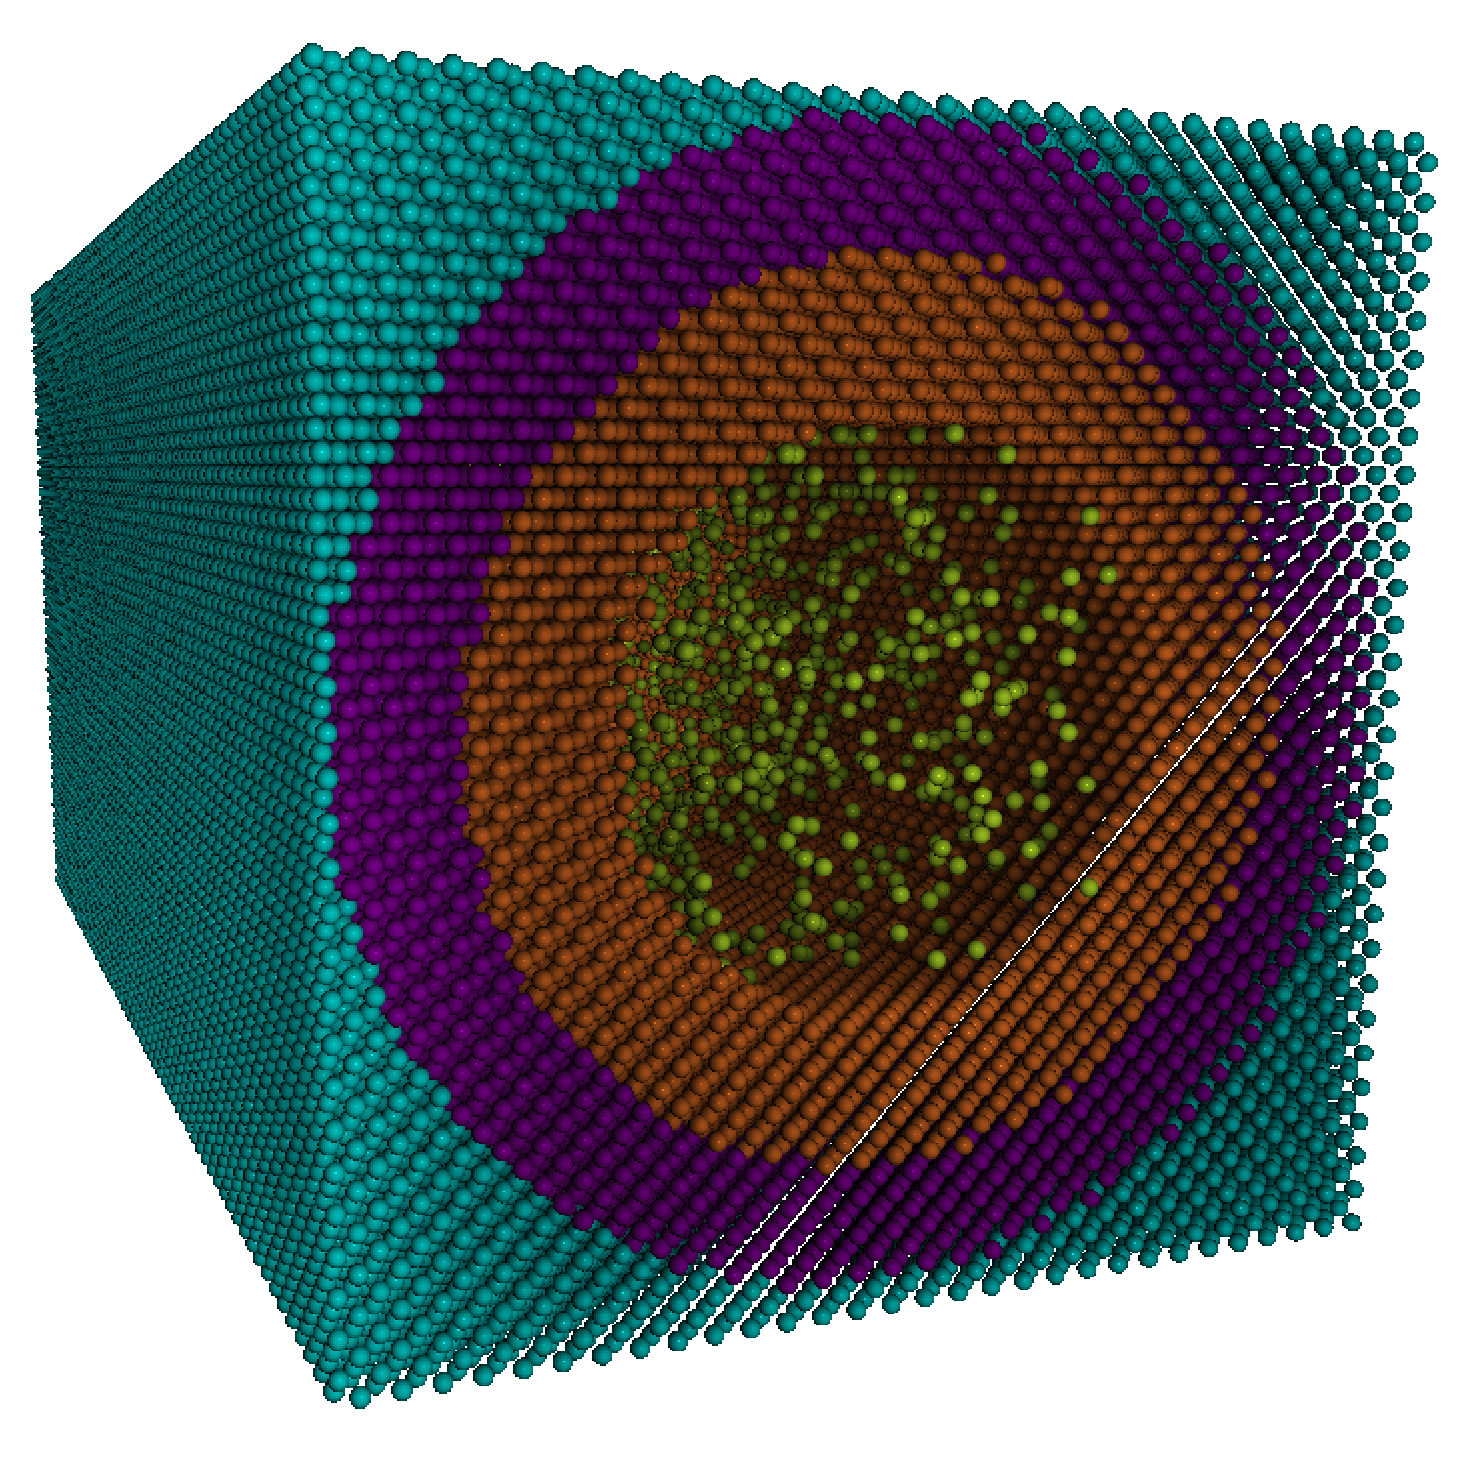
\includegraphics[width=0.5\textwidth]{lj_flow/configuration.png}
	\caption{
		Initial configuration in our case study simulation.
		A periodic box consisting of $(40\times25\times25)$ FCC unit cells with reduced density $\rho^* = 0.8442$ where we will have gas flow in a cylinder with radius 10 (reduced length).
		The different colors indicate the regions of which different integration rules apply.
		Blue atoms are fixed and do not move at all,
		whereas the yellow atoms are thermalized with a Langevin\citep{schneider1978molecular} dissipative thermostat to mimick the heat exchange with the frozen bulk atoms.
		The red and the green atoms are integrated normally, except the green gas atoms have an applied constant acceleration representing the pressure gradient.
		Setting up and verifying the system is simple using Atomify due to i.e. the real-time coloring of groups and regions.
    }
	\label{fig:cylinder_simulation}
\end{figure}

In this case study, we will use Atomify to measure the velocity profile of a
Lennard Jones gas inside a nanotube with varying density to observe
the slip velocity effect at low densities.

We create the nanotube inside a Lennard Jones solid of size  $(40\times25\times25)$ unit cells with reduced density $\rho^* = 0.8442$.
The fluid in the nanochannel, or cylinder, will flow due to an induced pressure gradient, see Fig. \ref{fig:cylinder_simulation}.
Here we apply a pressure gradient $\nabla P$ in the $x$-direction on the gas atoms using a constant acceleration $a$ calculated as
\begin{align}
	a = \frac{\nabla P}{\rho_m},
\end{align}
where $\rho_m$ is the mass density of the gas atoms.

Applying such an acceleration means adding energy to the system which in turn will increase the temperature and eventually melt the system.
To avoid this, we will couple the solid to an external heat bath so the added energy can be transferred out from the system through a dissipative thermostat.

Even though we only apply a pressure gradient on the gas atoms, the induced momentum will also be transferred to the solid atoms which eventually will start moving in the positive $x$-direction which is not desired.
We therefore freeze the outmost atoms (blue in Fig \ref{fig:cylinder_simulation}).
To obtain a system like this, we divide the atoms into multiple regions, which are integrated differently:

\begin{itemize}
	\item $r \leq 10$: applied pressure gradient
	\item $r \leq 17$: regular time integration
	\item $14 < r \leq 17$: Dissipative Langevin thermostat
	\item $17 < r$: frozen.
\end{itemize}
The different radii are specified in reduced Lennard Jones units.

\subsection{Creating the initial geometry}
We create a new script in Atomify using \keys{\cmd+N}, and save it (\keys{\cmd+S}) as \code{run.in}.
Start from the following input script
\lstinputlisting[language=LAMMPS]{simple.in}
we will modify it part by part.
Here, we have a Lennard Jones solid with reduced density
$\rho^* = 0.8442$, reduced mass $m^* = 1.0$ with $(40\times25\times25)$
FCC unit cells and a cutoff of $2.5\sigma$ where $\sigma$ is 1.0 in the reduced units.


To make sure LAMMPS executes our modifiction before visualization is started,
we need to make sure that additional commands happen \textit{before} the \code{run 1000} command.
If not, LAMMPS will run 1000 timesteps before getting to our modifications.

To define the inner cylinder, we first specify the radius and the center before using the region command
\begin{lstlisting}[basicstyle=\tiny, frame = none, numbers=none, framexleftmargin=0pt, xleftmargin=-0.75cm, xrightmargin=0.0cm]
	variable R equal $(ly*0.25)
	variable c equal $(ly*0.5)
	region cylinder1 cylinder x $c $c $R EDGE EDGE
\end{lstlisting}
The region command will create a cylinder $C_1$ in the $x$-direction, with $(y,z)$-coordinates at the system center \code{\$c} with radius \code{\$R} using the full length of the cylinder specified when using \code{EDGE}.

We now press \keys{\cmd+R} to run the simulation to see how it looks.
As shown in Fig. \ref{fig:rightbar}, we can hover the specified region to highlight the atoms in that region.

When we hover the region, we immediately see that the cylinder is in fact not placed at the center of the system, as shown in Fig. \ref{fig:initial_configuration}a.
The reason is that LAMMPS operate with two different units, either the length unit or the lattice length unit. This is explained in the documentation, but is a common mistake.
Discovering mistakes like this is very easy using Atomify.
The problem here is that LAMMPS expects the values to be in \textit{lattice} units, i.e. multiples of the lattice constant.
Since we used \code{\$(0.5*lx)} - which is in the actual lenght units - we need to specify \code{units box} in the region command.
We then rerun the simulation with \keys{\cmd+R} which gives the expected result in figure \ref{fig:initial_configuration}b.

\begin{figure}
	\centering
	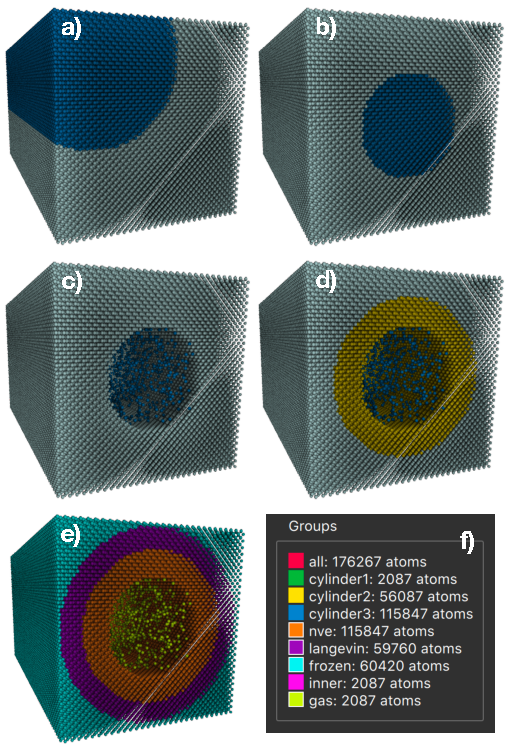
\includegraphics[width=0.5\textwidth]{figures/initial_configuration.pdf}
	\caption{
		Several snapshots of the process of creating the simulation in our case study.
		This shows how one typically generate a geometry step by step where the immediate
		feedback is very useful to quickly discover mistakes.
		The wrongly placed cylinder is shown in a) whereas it is placed correctly in b).
		c) shows how the system looks after deleting atoms to obtain $\rho = 0.01$. The next cylinder $C_2$ is shown in d),
		and all regions (placed in groups) are shown in e). Here we have uniquely defined the purple shell which should have a dissipative thermostat.
		In f), the list of all groups defined in this system is shown with colors matching those of e). All figures are rendered with Atomify.
    }
	\label{fig:initial_configuration}
\end{figure}
We now want to delete atoms so that we have a certain density. The volume of the inner cylinder is $\pi R^2 L$ which can be calculated in LAMMPS with \code{variable V equal PI*v\_R*v\_R*lx}.
We have chosen reduced mass units so the mass of our atoms is 1. The number density $\rho$ then equals the mass density $\rho_m$.
The command \code{delete\_atoms} can be used: \code{delete\_atoms porosity region-ID fraction seed}, where we need to specify the fraction of the existing atoms in that region we want to delete, and a random seed which can be any positive number.
Since we want to specify a certain density, we need to figure out how many atoms we should delete which depends on the current number of atoms inside the region.

To count the number of atoms inside a region, we first create a group containing all the atoms in it, and then create a variable that counts them.
Assuming density $\rho = 0.1$, we can calculate the expected number inside the cylinder as $N = V\rho$.
The atoms inside the region can now be deleted with the following commands
\begin{lstlisting}[basicstyle=\tiny, frame = none, numbers=none, framexleftmargin=0pt, xleftmargin=-0.75cm, xrightmargin=0.0cm]
	group cylinder1 region cylinder1
	variable N_cyl equal count(cylinder1)
	variable V equal PI*v_R*v_R*lx
	variable rho equal 0.1
	variable N_wanted equal $V*${rho}
	variable delete_fraction equal (${N_cyl}-${N_wanted})/${N_cyl}
	delete_atoms porosity cylinder1 ${delete_fraction} 1234
\end{lstlisting}
and the result is shown after rerunning again with \keys{\cmd+R}, see Fig. \ref{fig:initial_configuration}c.

This is a powerful workflow with Atomify where quick changes can be tested with immediate feedback.
Each time we add or change a command, we just rerun with \keys{\cmd+R} to see how it looks like.

The next step now is to create a larger cylinder $C_2$, the one containing the red atoms in Fig. \ref{fig:cylinder_simulation}, where regular time integration will take place.
This cylinder should have a slightly bigger radius and can be created with another region command:
\begin{lstlisting}[basicstyle=\tiny, frame = none, numbers=none, framexleftmargin=0pt, xleftmargin=-0.75cm, xrightmargin=0.0cm]
	region cylinder2 cylinder x $c $c $(v_R+4) EDGE EDGE
\end{lstlisting}
Again press \keys{\cmd+R} and see the expected result in Fig. \ref{fig:initial_configuration}d.

Now we have the inner cylinder with the gas atoms defined as a region and the next cylinder shell (including the gas atoms) defined as another region.
We now want to create another shell, the one with the dissipative thermostat.
All the atoms with the dissipative thermostat, the inner shell and the gas will be integrated with the \code{fix nve} integrator.
We therefore create a larger cylinder $C_3$ with $r=17$ which will be the one defining the group for \code{fix nve}.
With all three regions defined, we can also create groups which can be used in fixes
\begin{lstlisting}[basicstyle=\tiny, frame = none, numbers=none, framexleftmargin=0pt, xleftmargin=-0.75cm, xrightmargin=0.0cm]
	region cylinder3 cylinder x $c $c $(v_R+7) EDGE EDGE
	group cylinder1 region cylinder1
	group cylinder2 region cylinder2
	group cylinder3 region cylinder3
	group nve region cylinder3
\end{lstlisting}
where we also have created the group \code{nve} for clarity.

The dissipative thermostat will be \code{fix langevin}\citep{schneider1978molecular}, but it should only be applied on the outer shell defined by atoms being in $C_3$, but not in $C_2$.
Groups define sets on which we can apply regular set operations like union, intersection and subtraction.
We can obtain the outer shell with the command

\begin{lstlisting}[basicstyle=\tiny, frame = none, numbers=none, framexleftmargin=0pt, xleftmargin=-0.75cm, xrightmargin=0.0cm]
	group langevin subtract cylinder3 cylinder2
	group frozen subtract all cylinder3
	group gas dynamic all region cylinder1 every 1
\end{lstlisting}

We here also created the group \code{frozen}, which contains only the outmost atoms,
and the group \code{gas} which is dynamic since atoms may go in and out, and we want
to only apply a force on the ones in the inner cylinder $C_1$ at any point in time.
The frozen atoms will not move at all and make sure that the system does not start 
moving due to momentum transfer from the gas particles through the solid.

These groups are highlighted in Fig. \ref{fig:initial_configuration}e by hovering the box containing all the groups in Atomify as shown in Fig. \ref{fig:initial_configuration}f.
The colors of the atoms matches those in the group name in Fig. \ref{fig:initial_configuration}f, where the order of coloring is the same as they were defined in the script.
Although one group is colored green, we don't see any green atoms (\code{cylinder1}) since all of them also are in the groups \code{cylinder2}, \code{cylinder3}, \code{nve} and \code{gas},
so the color is overrided.

\subsection{Physical setup}
Now that we have achieved to set up the system geometrically, that is, all the different groups of atoms are defined.
We only need to apply the different actions, or fixes, on them.
First, we apply the time integration \code{fix nve} which should happen on all atoms within $C_3$, then the thermostat \code{fix langevin}

\begin{lstlisting}[basicstyle=\tiny, frame = none, numbers=none, framexleftmargin=0pt, xleftmargin=-0.75cm, xrightmargin=0.0cm]
	fix nve nve nve
	fix langevin langevin langevin 1.0 1.0 1.0 12345
	compute displacement all displace/atom
\end{lstlisting}

The syntax for fixes is \code{fix ID groupID style args}, so the above fixes have the same name as both the groups and the fix style.
\code{fix langevin} takes at least 4 arguments \textit{Tstart, Tstop, Tdamp, seed}, i.e. the temperature in the beginning of a simulation, the temperature at the end (timesteps in between get a linearly interpolated temperature between these values), a damping parameter which controls how strongly the thermal bath interacts with the system.
It also needs a random seed due to the random nature of the Langevin thermostat as discussed in \citep{schneider1978molecular}.
Finally, we have added another compute that measures the displacement per atom.
Hovering this compute in the list will color each atom according to their displacement since $t=0$.

By rerunning again (\keys{\cmd+R}), we can confirm that the system behaves as expected.
In Fig. \ref{fig:moving_atoms}, we see that the outmost atoms are completely frozen (dark blue), the ones in the solid are also blue, but brighter, since they vibrate thermally in the lattice.
The inner cylinder contains gas atoms which move more freely, as seen from the colors being in the upper part of the color map.

\begin{figure}
	\centering
	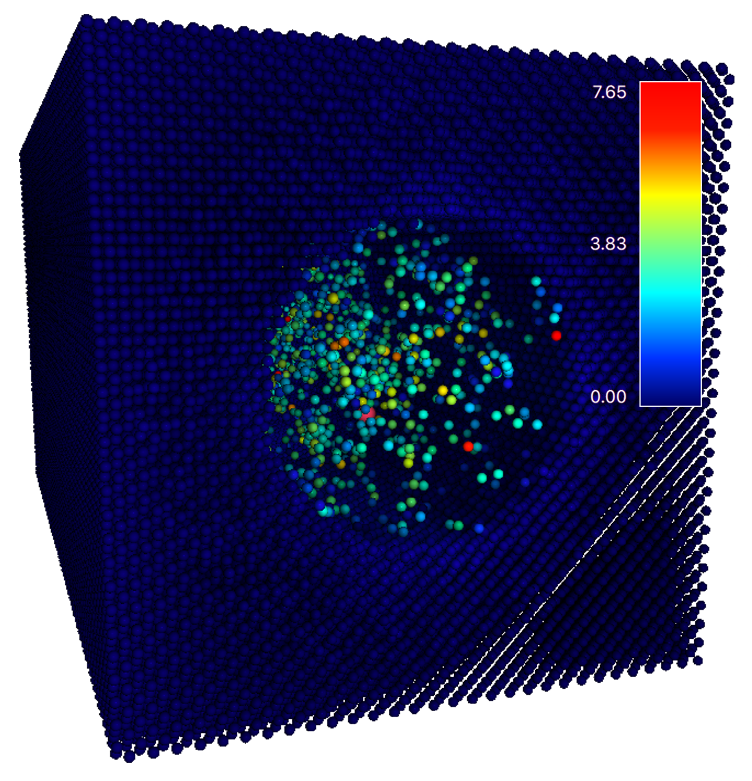
\includegraphics[width=0.5\textwidth]{lj_flow/07_moving.png}
	\caption{
		We see the expected moving atoms inside the $C_3$ cylinder.
		The atoms are colored based on their displacement (measured in reduced length units).
		We confirm that the outmost atoms are frozen, which we read from dark blue color mapping to 0 displacement.
		The moving atoms in the solid are blue, but brighter than the frozen ones which is expected due to their thermal vibrations.
		Inside the inner cylinder we see that the gas moves more freely since these atoms are not bounded.
    }
	\label{fig:moving_atoms}
\end{figure}

The only remaining part now is to set up the commands that will apply the pressure gradient and measure the radial velocity profile.

\subsection{Measurement setup}
We will use the built-in binning feature in LAMMPS called \textit{chunks}, a very general concept where you assign a \code{chunkID} to each atom
based on its position. LAMMPS supports multiple different \textit{chunk styles}, one of which is cylinder.
In the cylinder binning, we choose the same properties as for a cylinder region (center, length etc), but also the binsize in the length direction and how many radial bins we want.
We only want one bin in the flow direction since we will measure the radial velocity profile only.
The command for giving each atom a \code{chunkID} is\footnote{The \& is used to continue the command on the next line.}
\begin{lstlisting}[basicstyle=\tiny, frame = none, numbers=none, framexleftmargin=0pt, xleftmargin=-0.75cm, xrightmargin=0.0cm]
	compute chunk all chunk/atom bin/cylinder x lower &
	$(lx) $c $c 0 $R 30 units box
\end{lstlisting}
See the documentation for details about this command, but note that the binsize in the length direction is equal to the system length so we only get one bin.
It will create 30 radial bins for $r\in (0, R)$, where $R$ is the radius of the inner cylinder.
The final command we will use is the \code{fix ave/chunk} where we can get a smooth averaged velocity profile sampled over many timesteps.
To obtain this, we simply use
\begin{lstlisting}[basicstyle=\tiny, frame = none, numbers=none, framexleftmargin=0pt, xleftmargin=-0.75cm, xrightmargin=0.0cm]
	fix vx all ave/chunk 10 10 100 chunk vx ave running
\end{lstlisting}
Here we use every 10th value to sample the velocity profile, keeping all samples to sum them into a large histogram.
This fix will appear in the list of fixes in the Simulation summary just as groups, regions, computes and variables.
When we click it, we will get the figure shown in Fig. \ref{fig:velocity_profile1}.

\begin{figure}
	\centering
	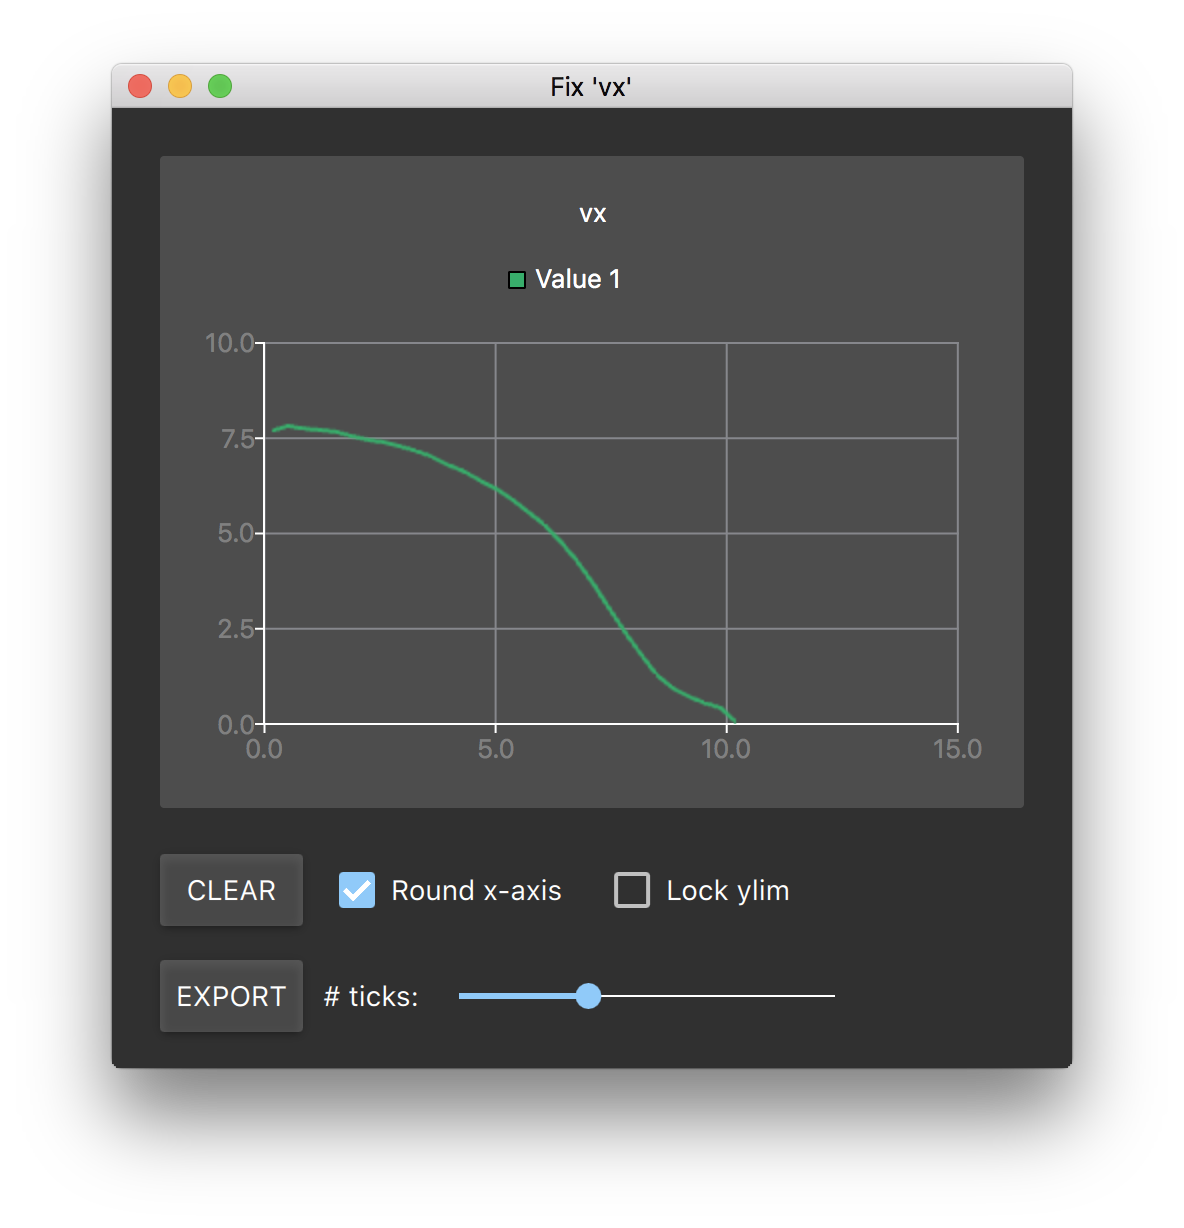
\includegraphics[width=0.5\textwidth]{lj_flow/08_velocity_profile1.png}
	\caption{
		The velocity profile for a Lennard Jones gas inside a nanochannel of radius 8.7 (reduced units).
		Since the wall also is made of Lennard Jones atoms, some of the wall atoms
		This figure is made using the Atomify real-time plotter which can show any scalar value defined in LAMMPS
		as compute, fix or variable.
    }
	\label{fig:velocity_profile1}
\end{figure}

\subsection{Results}

\begin{figure}
	\centering
	% 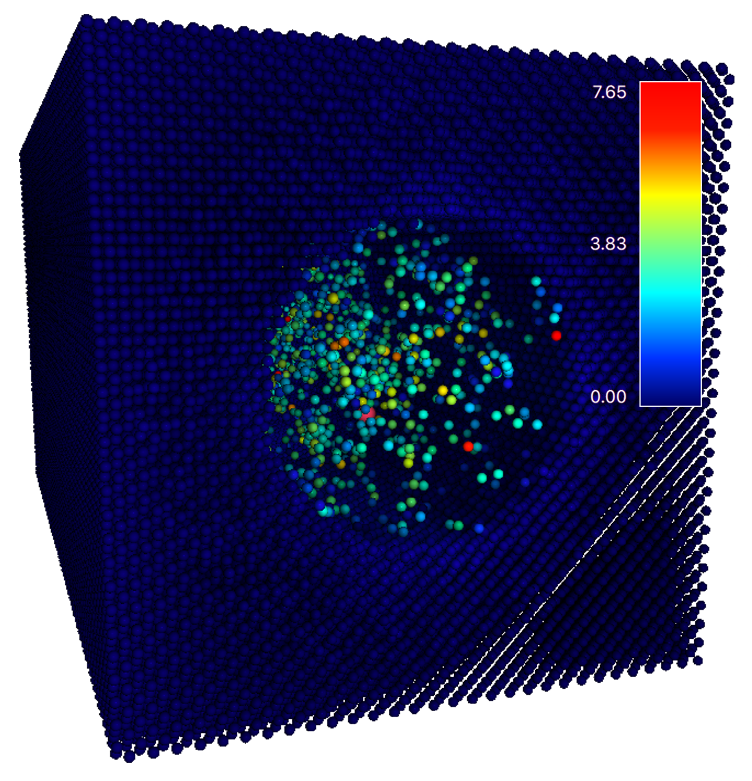
\includegraphics[width=0.5\textwidth]{lj_flow/07_moving.png}
	\caption{
		Velocity profiles for different densities.
		The step flow shape is evident for low density gases with a high non-zero slip velocity.
		When the density increases, the slip velocity goes to zero as expected.
    }
	\label{fig:velocity_profiles}
\end{figure}

We conclude this case study with a series of simulations of the system described above for different densities $\rho$.
Each simulation runs 10000 timesteps before we export the plots from \code{fix vx} to MATLAB using the Export function seen in Fig. \ref{fig:velocity_profile1}.
All these plots are now merged into a final figure which is shown in Fig. \ref{fig:velocity_profiles}.
It is here evident that the velocity near the boundary is not zero, which is the reason why the permeability is much higher for dilute gases than dense liquids.
This is, as mentioned earlier, called the Klinkenberg effect\citep{klinkenberg1941permeability}.

\section{\label{sec:discussion}Discussion}
In this paper we have presented Atomify, an application that reduces the large amount of context switches and mouse clicks
when creating new simulation scripts.
As of today, only LAMMPS is supported as the physical simulator, but other codes can easily be integrated
due our general implementation with no assumpetion about the underlying code except atom positions.
The communication overhead is minimized since LAMMPS runs in the same process as Atomify, sharing the memory.

\section{\label{sec:future}Future work}
Atomify continues in heavy development and we have several features planned for future versions.
We already have a simple version of Atomify in the web browser using WebGL and WebAssembly.
This makes it easy to test scripts in the browser with all simple functionalities available.
This is especially useful in educational settings where teachers wish to introduce students
to LAMMPS without installing additional software.
It will also serve as a nice demonstration of the full desktop application of Atomify.

\section{Availability}
Atomify is availabe on Linux, MacOS and Windows and can be downloaded from
\href{https://ovilab.net/atomify}{http://ovilab.net/atomify}.
A lightweight version of Atomify is also available for mobile devices running
Android or iOS.

\section{Acknowledgments}

\section{Disclosure}

Svenn-Arne Dragly is employed part-time by The Qt Company.

\bibliography{Remote}

\end{document}
